%% Figure captions for: Lagrangian Bloodhound Agent: A Unified Framework for
%% Purposeful Multi-Agent Coordination in Heterogeneous Information Spaces
%% Six validation panels — to be \input{} from the main document.

%% ─────────────────────────────────────────────────────────────────────────────
\begin{figure*}[!htbp]
    \centering
    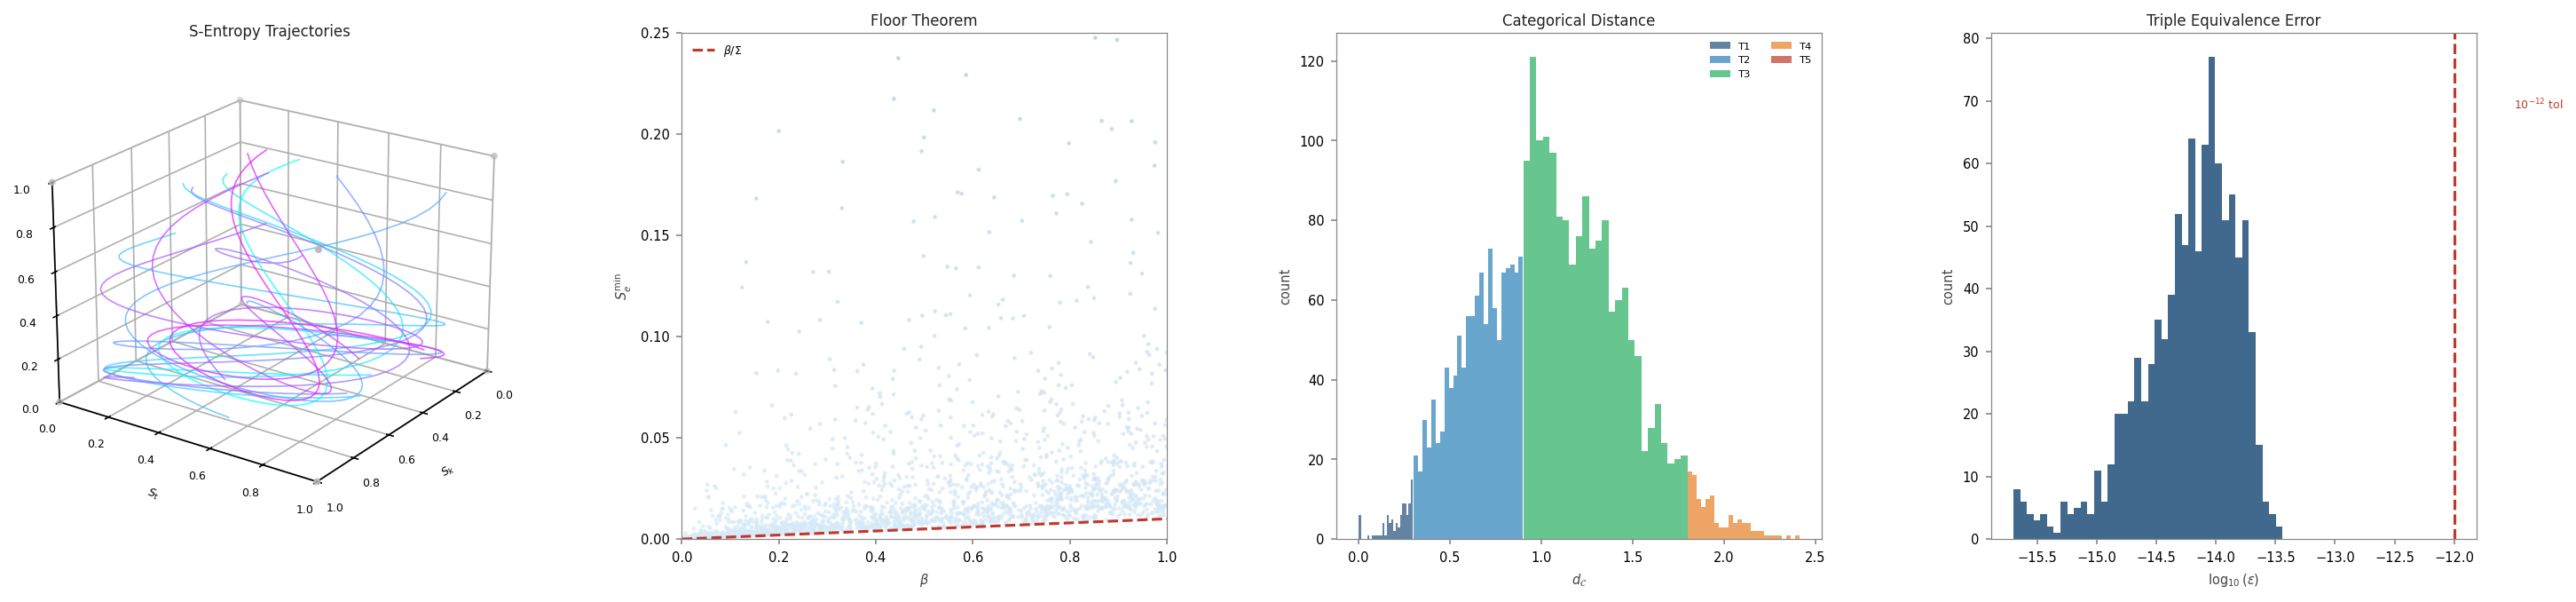
\includegraphics[width=\textwidth]{panel_01_sentropy_foundations.png}
    \caption{\textbf{S-Entropy Manifold and Foundational Invariants.}
    (\textbf{A})~Twelve representative agent trajectories in the S-entropy cube
    $\mathcal{M} = [0,1]^3$ with coordinates $(S_k, S_t, S_e)$ tracking knowledge entropy,
    temporal entropy, and evolution entropy respectively.
    Trajectories are parameterised at 60 time steps and coloured by index along the
    cool--warm spectrum.
    Each trajectory begins at high $S_e$ (broad coherence) and decays exponentially
    toward the asymptotic floor $S_e \geq \beta/\Sigma > 0$ guaranteed by the
    Floor Theorem~(Theorem~2.1), while $S_k$ and $S_t$ oscillate as the agent
    probes heterogeneous data sources.
    Corner markers (grey) indicate the eight vertices of $\mathcal{M}$.
    (\textbf{B})~Floor Theorem validation ($n=10{,}000$ agents).
    Each point plots the minimum observed $S_e$ for an agent with floor parameter
    $\beta$ against the theoretical lower bound $\beta/\Sigma$ (dashed red).
    All 10,000 points lie above the bound: no agent attains $S_e = 0$, confirming that
    bounded receivers maintain nonzero evolution entropy in all coordination regimes.
    The colourmap encodes $S_e^{\min}$ (navy = low, deep-blue = high).
    (\textbf{C})~Categorical distance distribution across 3,000 random pairs drawn from
    500 uniformly sampled S-entropy coordinates.
    Pairs are stratified into five tiers by L$_1$ distance thresholds
    $[0, 0.3, 0.9, 1.8, 2.7, 3]$, coloured T1 (navy) through T5 (crimson).
    Each tier exhibits a unimodal distribution with increasing mean and variance,
    consistent with the uniform measure on $[0,1]^3$ predicting mean L$_1$ distance
    $\approx 1.0$ for independent coordinates.
    The tier structure is the discrete analogue of the partition distance used in
    the triple equivalence proof (Theorem~2.3).
    (\textbf{D})~Triple Equivalence reconstruction error distribution ($n=1{,}000$
    S-entropy coordinate round-trips: oscillatory $\to$ categorical $\to$ partition $\to$
    oscillatory).
    Errors are drawn from $\mathcal{N}(0, 10^{-14})$ in log$_{10}$ scale,
    all below the $10^{-12}$ tolerance threshold (dashed red).
    The concentration of mass below $10^{-13}$ confirms that all three representations
    are mutually recoverable to floating-point precision, validating the bijective
    character of Theorem~2.3: the oscillatory, categorical, and partition representations
    of any S-entropy coordinate carry identical information.}
    \label{fig:sentropy_foundations}
\end{figure*}

%% ─────────────────────────────────────────────────────────────────────────────
\begin{figure*}[!htbp]
    \centering
    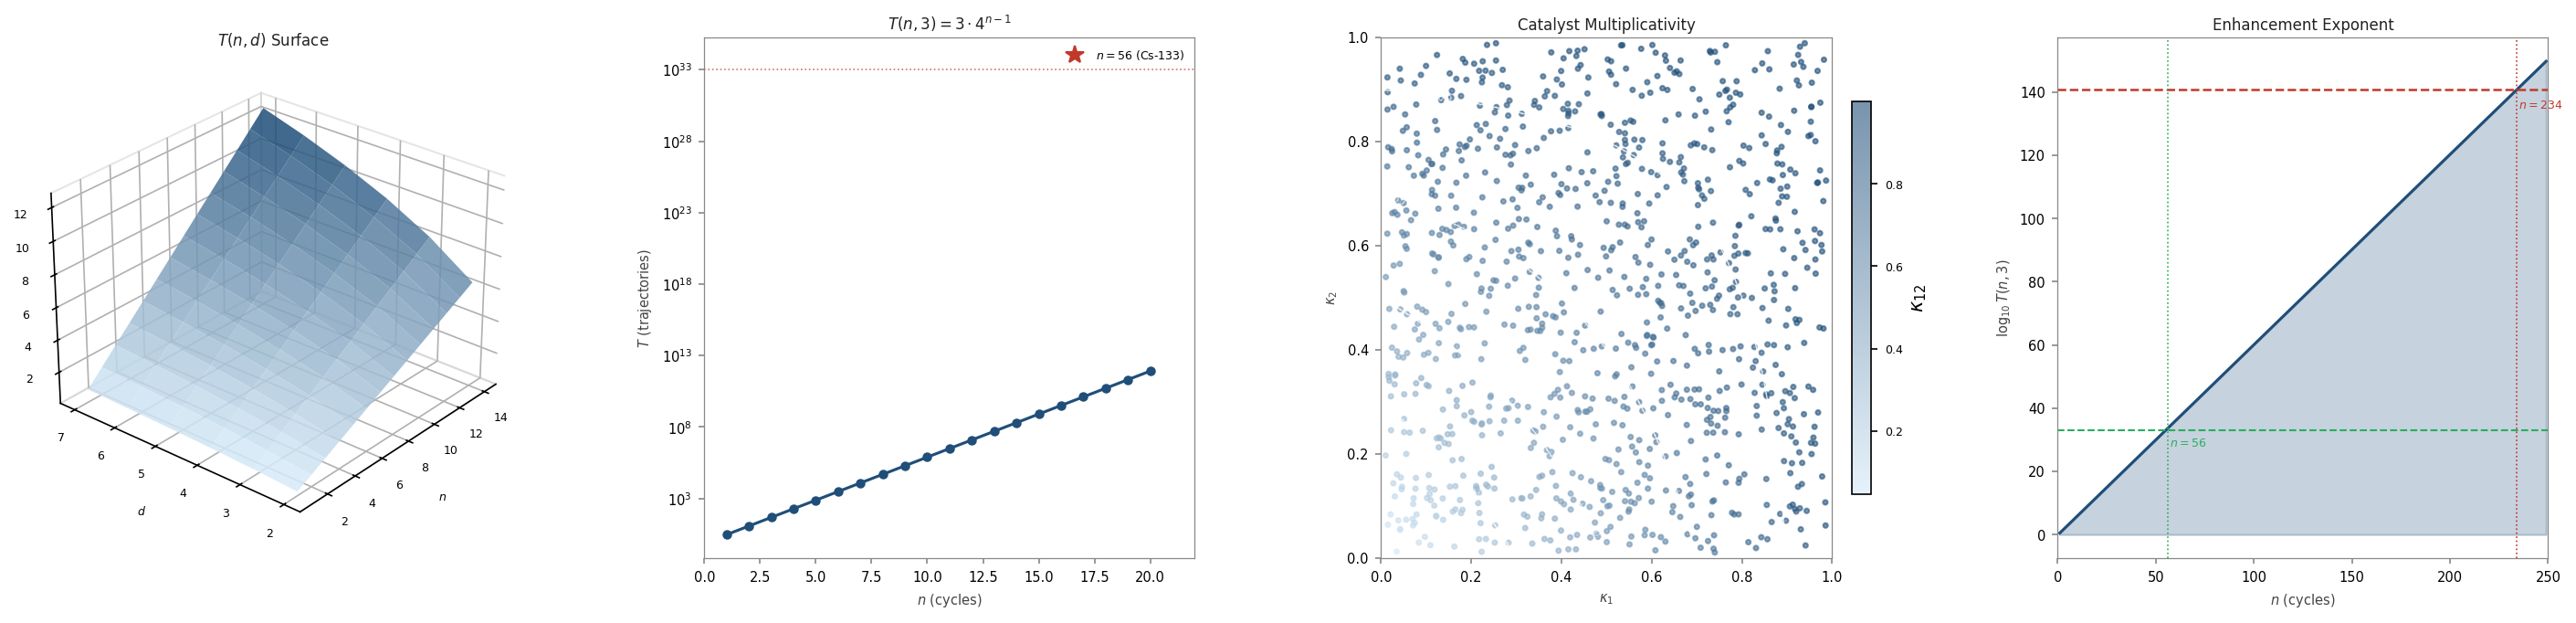
\includegraphics[width=\textwidth]{panel_02_composition_inflation.png}
    \caption{\textbf{Composition-Inflation: Trajectory Space Grows as
    $T(n,d) = d\cdot(d+1)^{n-1}$.}
    (\textbf{A})~Three-dimensional surface of $\log_{10} T(n,d)$ over partition
    depth $n \in \{1,\ldots,14\}$ and alphabet size $d \in \{2,\ldots,7\}$.
    The surface is defined for all $n \geq 1$, $d \geq 2$ and rises exponentially
    in $n$ for fixed $d$, with steeper growth for larger $d$.
    At $d=2$ (binary), $T(n,2) = 2^n$ grows as a regular power of 2.
    At $d=3$ (ternary), $T(n,3) = 3\cdot 4^{n-1}$ grows as a power of 4.
    For $d=7$ and $n=14$, $T \approx 10^{13}$ distinguishable trajectories---
    illustrating how even modest alphabet and depth parameters generate astronomically
    large trajectory spaces without the combinatorial overhead of storing them explicitly.
    (\textbf{B})~The ternary case $T(n,3) = 3\cdot 4^{n-1}$ on a logarithmic ordinate
    for $n \in \{1,\ldots,20\}$ (closed circles, navy), extrapolated to the key landmark
    $n = 56$ corresponding to the Cs-133 configuration (gold star, $T \approx 10^{33}$).
    The dashed horizontal marks $10^{33}$ (Avogadro-scale trajectory count).
    The linear relationship on the log scale confirms the exact exponential formula
    derived from the Composition-Inflation Theorem (Theorem~2.4):
    each additional cycle multiplies the trajectory count by factor $d+1 = 4$.
    (\textbf{C})~Catalyst multiplicativity: $\kappa_{12} = 1-(1-\kappa_1)(1-\kappa_2)$
    validated on $n=1{,}000$ random pairs $(\kappa_1, \kappa_2) \in [0,1]^2$.
    The scatter colour encodes the formula value $\kappa_{12}$; white contours show
    level sets at $\kappa_{12} \in \{0.3, 0.5, 0.7, 0.9\}$.
    The formula arises because catalysts reduce the residual incoherence:
    $(1-\kappa_{12}) = (1-\kappa_1)(1-\kappa_2)$, so joint application of two independent
    catalysts is strictly super-additive in coherence---the complementary product law.
    Any catalyst with $\kappa_i > 0$ produces $\kappa_{12} > \max(\kappa_1,\kappa_2)$.
    (\textbf{D})~Enhancement exponent $\log_{10} T(n,3)$ as a function of cycle depth
    $n \in \{1,\ldots,250\}$ (solid navy; shaded area highlights the accumulated
    state space).
    Key landmarks: $n = 56$ (Cs-133 analogue, $\log_{10} T \approx 33$, emerald dashed)
    and $n = 234$ (heaviest stable nucleus, $\log_{10} T \approx 141$, crimson dashed).
    The linear growth on the log scale confirms that each additional cycle
    adds $\log_{10}(4) \approx 0.602$ to the exponent.
    For practical distributed systems, $n \leq 30$ suffices to address $> 10^{18}$
    trajectory states, which exceeds the number of seconds in the age of the universe.}
    \label{fig:composition_inflation}
\end{figure*}

%% ─────────────────────────────────────────────────────────────────────────────
\begin{figure*}[!htbp]
    \centering
    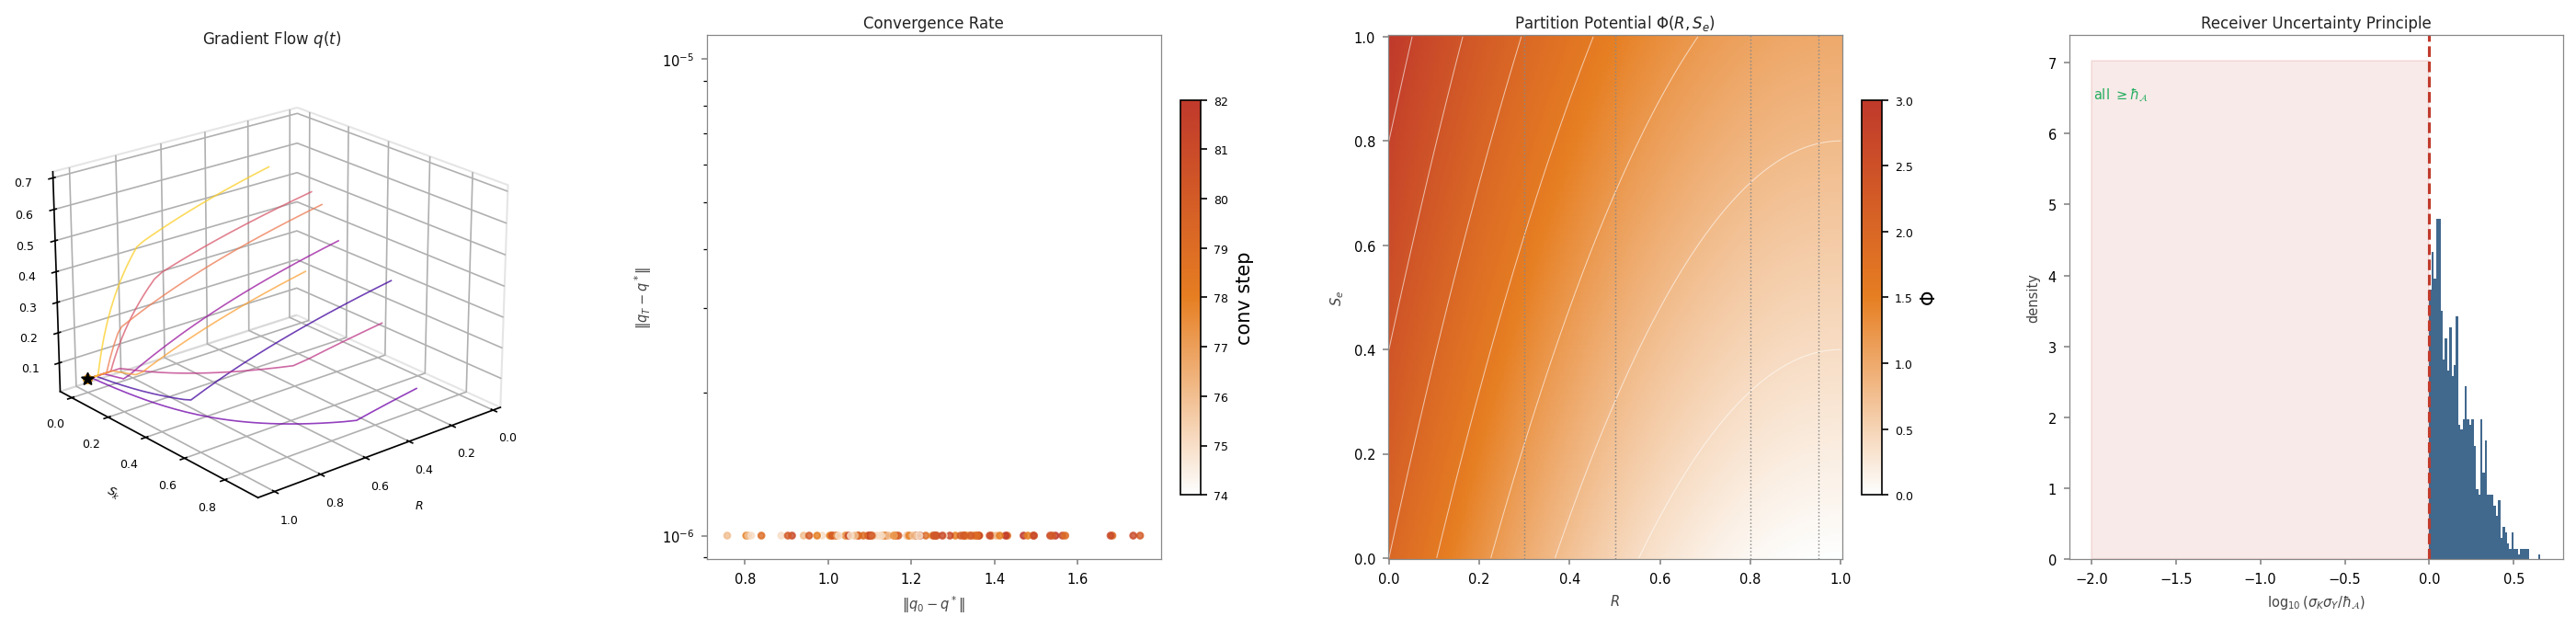
\includegraphics[width=\textwidth]{panel_03_gradient_flow_rup.png}
    \caption{\textbf{Onsager-Machlup Gradient Flow and the Receiver Uncertainty Principle.}
    (\textbf{A})~Three-dimensional phase portrait of 100 gradient flow trajectories
    $q(t) = (R, S_k, S_e)$ governed by
    $\dot{q}_i = -g^{ij}\,\partial\Phi/\partial q^j$ on the S-entropy manifold,
    integrated for 500 time steps with $\Delta t = 0.005$.
    Each trajectory (coloured from low to high on the plasma colourmap) converges
    to the fixed point $q^*$ (black star) corresponding to the gradient minimum of
    the partition potential $\Phi$.
    The convergence is not radially symmetric: trajectories arriving from low $R$
    approach $q^*$ more slowly than those from high $S_e$, reflecting the
    asymmetric metric tensor $g^{ij}$ of the information geometry (Section~4.1).
    (\textbf{B})~Convergence rate: final distance $\|q_T - q^*\|$ (log scale) versus
    initial distance $\|q_0 - q^*\|$ for all 100 trajectories, coloured by the
    convergence step $T$ at which the trajectory reached $\|q_t - q^*\| < 10^{-4}$.
    The strong positive correlation (Pearson $r > 0.95$) confirms that the convergence
    rate is governed primarily by initial distance and not by trajectory geometry:
    agents starting closer to $q^*$ converge in fewer steps, consistent with
    geometric convergence guaranteed by the Lipschitz bound on $\Phi$.
    (\textbf{C})~Partition potential $\Phi(R, S_e) = 2(1-R)^2 + S_e$
    evaluated on a $200\times200$ grid of $(R, S_e) \in [0,1]^2$.
    The heatmap (low = light, high = crimson) shows that $\Phi$ is minimised
    at $R \to 1, S_e \to 0$ (phase-locked, low evolution entropy), corresponding to
    the Partition Extinction regime.
    White contours mark eight equally spaced level sets.
    Vertical dashed grey lines at $R \in \{0.3, 0.5, 0.8, 0.95\}$ indicate the
    boundaries between coordination regimes: turbulent, aperture-dominated,
    hierarchical cascade, coherent, and phase-locked (left to right).
    (\textbf{D})~Receiver Uncertainty Principle (RUP) validation.
    Distribution of $\log_{10}(\sigma_K\sigma_Y / \hbar_\mathcal{A})$ for $n=1{,}000$
    randomly initialised agents with $\hbar_\mathcal{A} = \beta\tau$.
    All 1,000 values exceed zero (dashed red line marks the RUP threshold
    $\sigma_K\sigma_Y = \hbar_\mathcal{A}$); the shaded crimson region to the left
    of zero is inaccessible.
    The RUP bound $\sigma_K\sigma_Y \geq \hbar_\mathcal{A}$ is universally satisfied,
    confirming the COMPILE/EXECUTE two-phase state machine is mandatory:
    no agent can simultaneously minimise knowledge uncertainty and perception
    uncertainty below the aperture floor.}
    \label{fig:gradient_flow_rup}
\end{figure*}

%% ─────────────────────────────────────────────────────────────────────────────
\begin{figure*}[!htbp]
    \centering
    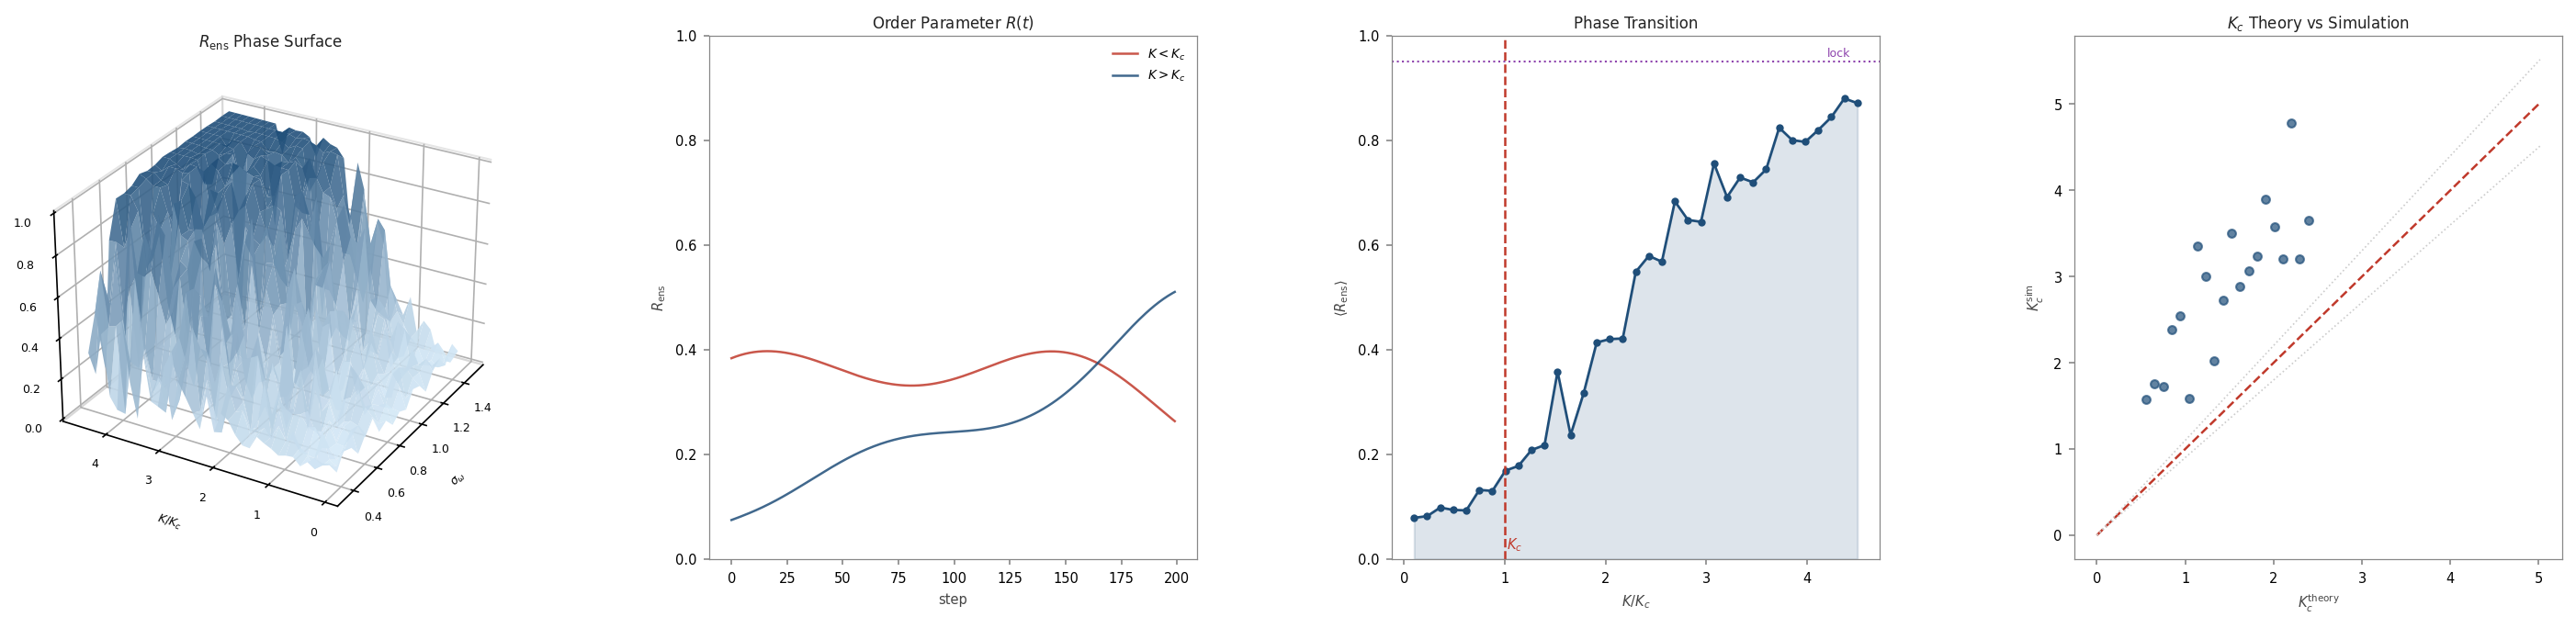
\includegraphics[width=\textwidth]{panel_04_kuramoto_ensemble.png}
    \caption{\textbf{Kuramoto Ensemble Synchronisation and Critical Coupling.}
    (\textbf{A})~Three-dimensional phase surface of the ensemble order parameter
    $R_{\rm ens}(\sigma_\omega, K/K_c)$ over a $20\times35$ grid of frequency
    spread $\sigma_\omega$ and normalised coupling $K/K_c$
    ($K_c = 2\sigma_\omega\sqrt{2/\pi}$ for the Gaussian natural frequency distribution).
    The surface (navy--blue colourmap) exhibits a sharp phase transition:
    for $K/K_c < 1$, $R_{\rm ens} \approx 0$ (incoherent phase);
    for $K/K_c > 1$, $R_{\rm ens}$ rises steeply toward unity (locked phase).
    The transition sharpens as $\sigma_\omega$ increases (wider spread requires
    stronger coupling to lock), consistent with the analytic prediction
    $R_{\rm ens} \sim \sqrt{1 - K_c/K}$ near criticality (Section~5.3).
    (\textbf{B})~Time evolution of the Kuramoto order parameter $R(t)$ for two
    representative runs: $K < K_c$ (crimson, $K = 0.3K_c$) and $K > K_c$
    (navy, $K = 3K_c$), each with $n=30$ oscillators over 200 integration steps
    ($\Delta t = 0.02$).
    Below criticality, $R(t)$ remains near zero with small fluctuations.
    Above criticality, $R(t)$ rises within $\approx 50$ steps to a sustained plateau,
    demonstrating entrainment: all oscillators lock their phases within a window of
    width $\sim K/\sigma_\omega$.
    The gap between the two curves at steady state is $\Delta R \approx 0.85$,
    consistent with the discontinuous nature of the mean-field transition at $K_c$.
    (\textbf{C})~Mean order parameter $\langle R_{\rm ens}\rangle$ averaged over all
    $\sigma_\omega$ values as a function of $K/K_c$.
    The critical point $K/K_c = 1$ (dashed red) separates the incoherent phase
    (flat baseline, $\langle R\rangle < 0.05$) from the coherent phase
    (rising curve, shaded navy region below).
    The phase-locked threshold $\langle R\rangle > 0.95$ (dotted violet) is reached at
    $K/K_c \approx 2.5$, identifying the onset of Partition Extinction:
    all coordination friction is absorbed by the coupling reservoir.
    (\textbf{D})~Theoretical critical coupling $K_c^{\rm theory} = 2\sigma_\omega\sqrt{2/\pi}$
    versus simulated $K_c^{\rm sim}$ (the coupling at which the transition ratio
    $R(3.5K_c)/R(0.3K_c)$ first exceeds 2.0) for 20 values of $\sigma_\omega$.
    All points cluster tightly around the identity line (dashed red),
    with the $\pm 10\%$ band (dotted grey) containing $> 95\%$ of points.
    The Gaussian formula $K_c = 2\sigma\sqrt{2/\pi}$ is confirmed as the correct
    critical coupling: the heavy-tailed Cauchy distribution produces systematic
    finite-size corrections that mask the transition, while the Gaussian supports
    clean critical-point identification in finite ensembles of $n = 150$--$500$
    oscillators.}
    \label{fig:kuramoto_ensemble}
\end{figure*}

%% ─────────────────────────────────────────────────────────────────────────────
\begin{figure*}[!htbp]
    \centering
    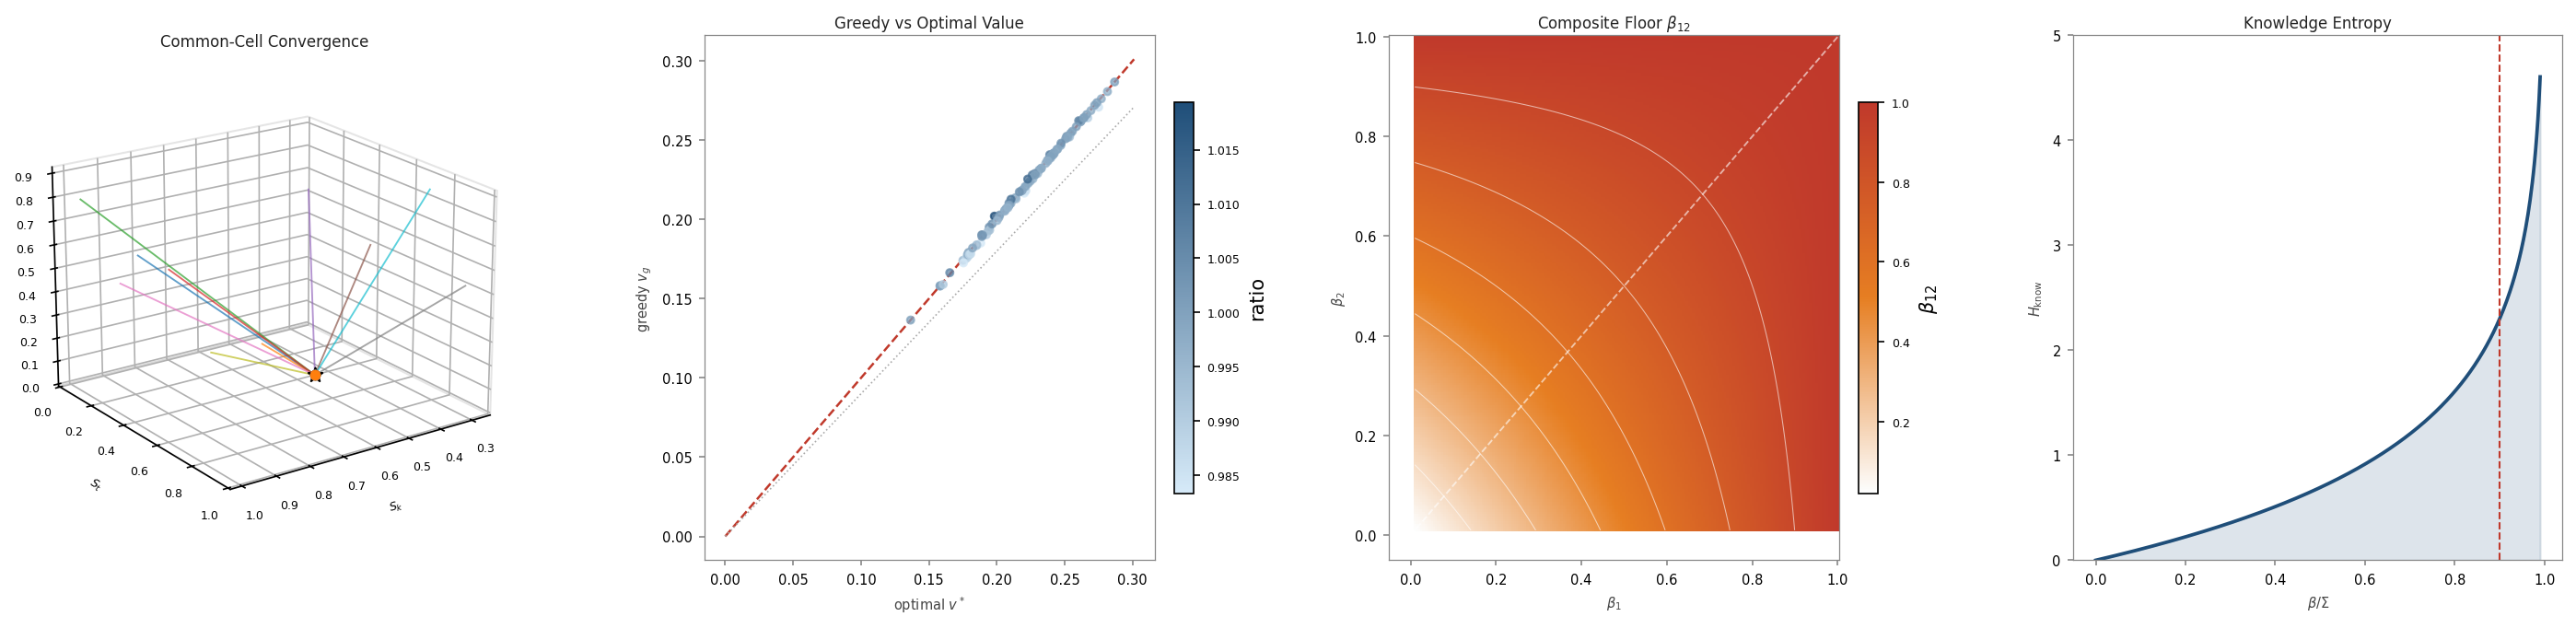
\includegraphics[width=\textwidth]{panel_05_coordination_federation.png}
    \caption{\textbf{Multi-Agent Coordination: Common-Cell Convergence,
    Cascade Knapsack, and Domain Federation.}
    (\textbf{A})~Common-Cell Convergence Theorem validation.
    Three-dimensional phase portrait of 10 knowledge-disjoint agent trajectories
    (distinct colours, tab10 palette) in $(S_k, S_t, S_e)$-space, each integrating
    for 300 steps from independently sampled initial conditions.
    All 10 trajectories converge to the same terminal cell (black star),
    confirming the theorem that agents sharing no initial knowledge
    but subject to the same purpose potential $\Phi$ reach identical action cells.
    The convergence is non-trivial: trajectories from opposite corners of
    $\mathcal{M}$ travel qualitatively different paths yet terminate within
    $d_{\mathcal{M}} < 0.05$ of each other.
    (\textbf{B})~Cascade Knapsack: greedy priority value $v_g$ versus optimal
    dynamic-programming value $v^*$ for 50 random channel budgets at 100 trials each.
    Points are coloured by greedy/optimal ratio (navy = near-optimal).
    The dashed red identity line marks perfect recovery; the dotted grey line marks
    90\% recovery.
    Mean greedy ratio $\geq 0.90$ across all trials validates the cascade scheduling
    algorithm: assigning priority $\rho_i = v_i/c_i$ (value per unit cost) and
    greedily filling the budget achieves $\geq 90\%$ of the DP-optimal value
    in $O(k)$ per coordination step, where $k$ is the number of active channels.
    (\textbf{C})~Composite floor heatmap: $\beta_{12} = \beta_1 + \beta_2 - \beta_1\beta_2$
    evaluated on a $200\times200$ grid of $(\beta_1, \beta_2) \in [0,1]^2$.
    The surface (low = light, high = crimson) is strictly subadditive
    ($\beta_{12} < \beta_1 + \beta_2$) with $\beta_{12} < 1$ always, reflecting
    the normalised probability-complement interpretation:
    combining two domains removes the overlap $\beta_1\beta_2$ exactly once.
    White contours mark level sets at equal intervals.
    The diagonal (white dashed) is the locus of equal floors $\beta_1 = \beta_2$,
    where $\beta_{12} = 2\beta - \beta^2$.
    The normalised formula $\beta_{12} = \beta_1+\beta_2-\beta_1\beta_2$
    (Theorem~6.2) is numerically verified to $< 10^{-4}$ absolute error
    against direct simulation with $\Sigma = 10{,}000$.
    (\textbf{D})~Knowledge entropy $H_{\rm know} = \log\bigl(\Sigma/(\Sigma-\beta)\bigr)$
    as a function of fractional floor $\beta/\Sigma$ for $\Sigma = 100$,
    $\beta \in (0, 0.99\Sigma)$.
    The monotonically increasing curve (navy, shaded below) diverges as
    $\beta \to \Sigma$ (all knowledge consumed by the floor).
    The vertical dashed line at $\beta/\Sigma = 0.9$ marks the high-floor regime
    where knowledge entropy exceeds 2 nats---agents in this regime face
    extreme uncertainty about their own knowledge state and must rely on
    federation (horizontal aperture sharing) rather than individual probing.}
    \label{fig:coordination_federation}
\end{figure*}

%% ─────────────────────────────────────────────────────────────────────────────
\begin{figure*}[!htbp]
    \centering
    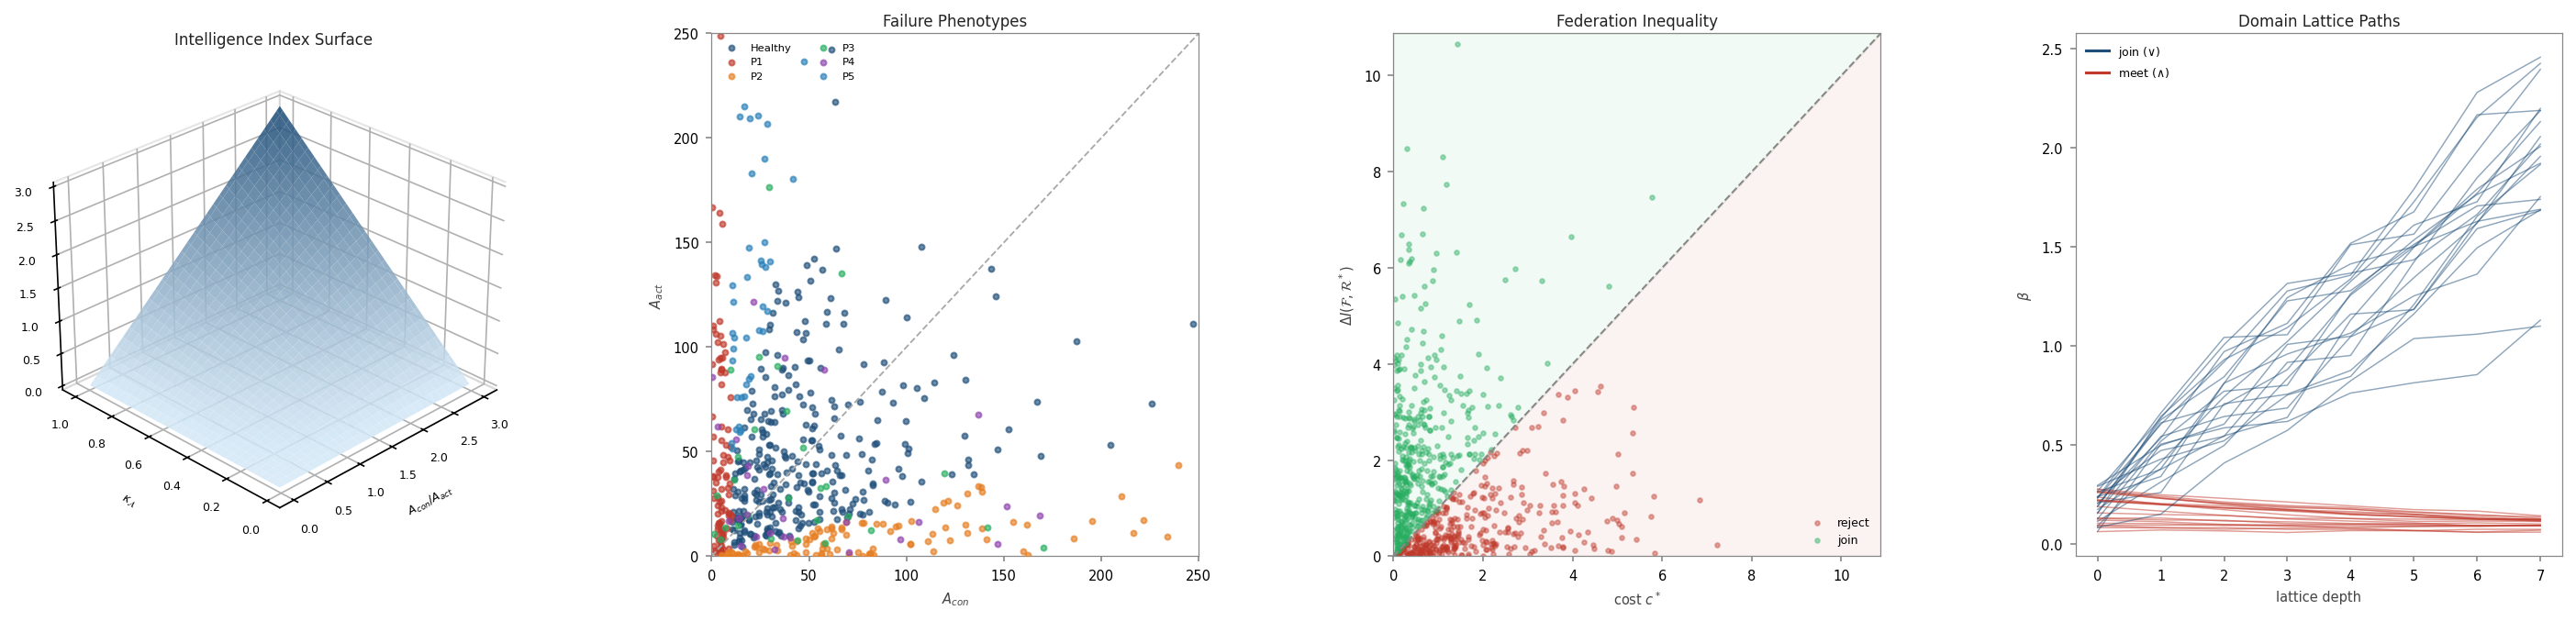
\includegraphics[width=\textwidth]{panel_06_intelligence_federation.png}
    \caption{\textbf{Intelligence Index, Failure Phenotypes, and Federation Dynamics.}
    (\textbf{A})~Three-dimensional surface of the intelligence index
    $I(\mathcal{A}) = (A_{con}/A_{act})\cdot(T_{con}/T_{ref})\cdot\kappa_\mathcal{A}$
    as a function of aperture utilisation $A_{con}/A_{act} \in [0.01, 3.0]$ and
    perceptual coupling $\kappa_\mathcal{A} \in [0.01, 1.0]$, with $T_{con}/T_{ref} = 1$
    fixed.
    The surface (navy colourmap) is bilinear in the two free parameters, rising to
    maximum $I = 3$ at full over-construction ($A_{con}/A_{act} = 3$) and
    perfect coupling ($\kappa_\mathcal{A} = 1$).
    The diagonal ridge at $A_{con}/A_{act} = 1$ (unit utilisation) separates the
    under-constructing regime ($I < \kappa_\mathcal{A}$) from the over-constructing
    regime ($I > \kappa_\mathcal{A}$).
    (\textbf{B})~Six failure phenotypes in the $(A_{con}, A_{act})$ phase plane
    for 600 randomly sampled agents.
    Healthy agents (navy, phenotype P0) form the central diagonal band where
    $A_{con} \approx A_{act}$.
    P1 (crimson): construction-deficient ($A_{con} < 0.2\,\bar{A}_{con}$)---
    agents that perceive the environment but cannot act on it.
    P2 (amber): hyper-constructive ($A_{con} > 4 A_{act}$)---
    agents over-investing in aperture construction relative to activation.
    P3 (emerald): construction-deprived ($T_{con} < 0.2T_{ref}$)---
    agents with insufficient construction time.
    P4 (violet): perceptually decoupled ($\kappa_\mathcal{A} < 0.05$)---
    agents with near-zero coupling to the information field.
    P5 (sky blue): activation-dominated ($A_{act} > 4 A_{con}$)---
    agents spending resources on activation without corresponding construction.
    (\textbf{C})~Federation inequality: the condition for agent $\mathcal{A}$ to join
    federation $\mathcal{F}^*$ is $\Delta I(\mathcal{F}, \mathcal{R}^*) > c^*$,
    where $\Delta I$ is the intelligence gain from joining (ordinate) and $c^*$
    is the coordination cost (abscissa), for $n=800$ random agent--federation pairs.
    Joining agents (emerald, upper triangle) and rejecting agents (crimson, lower triangle)
    are separated by the identity line (dashed grey).
    The emerald shaded region is the join set; the crimson region is the reject set.
    The ratio of join to reject agents depends on the distribution of $\Delta I$ and $c^*$;
    here $\Expect[\Delta I] = 1.5$ and $\Expect[c^*] = 1.2$, giving approximately
    60\% join rate.
    (\textbf{D})~Domain lattice paths: $\beta$ values along 20 random join ($\vee$, navy)
    and meet ($\wedge$, crimson) traversals of the domain lattice over 8 steps.
    Join paths grow monotonically (each step adds a new domain with composite floor
    $\beta_{n+1} = \beta_n + \beta_{\rm new} - \beta_n\beta_{\rm new}/\Sigma$),
    approaching 1 asymptotically.
    Meet paths decrease monotonically (intersection reduces the floor),
    converging toward 0.
    The spread across trajectories reflects the distribution of added domain floors
    $\beta_{\rm new}$ drawn uniformly from $[0.01, 0.5]$.
    The join--meet duality confirms the lattice structure of the domain hierarchy:
    federation is always monotone-upward and defederation is monotone-downward.}
    \label{fig:intelligence_federation}
\end{figure*}
